% !TEX root = ../main.tex
% Chapter Experiments results

\chapter{Results} % Main chapter title
\label{Chapter4} % Change X to a consecutive number; for referencing this chapter elsewhere, use \ref{ChapterX}

The main experiments' results are presented in this chapter. The different models trained and their results are explicitly detailed in Appendix~\ref{AppendixB}.


\section{Data preprocessing}
Raw string sentence is preprocessed in order to give the encoder, and the decoder, a tokenized sequence. There are different steps to prepare data for training and these steps are illustrated in Figure~\ref{fig:preprocess}. First, the raw sentence is tokenized to separate words and punctuation, the casing is not changed because it carries different information (e.g. start of sentence).

\begin{figure}
    \centering
    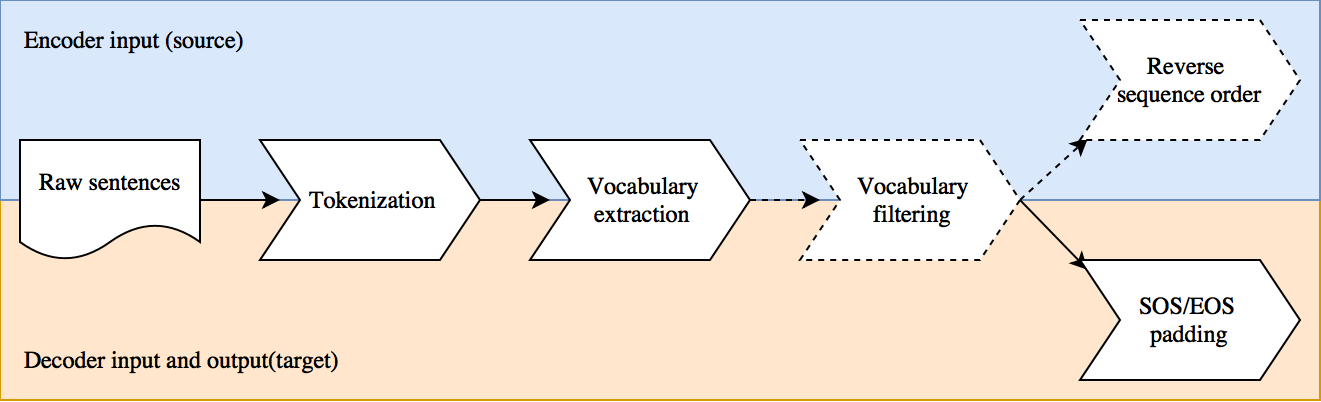
\includegraphics[width=\textwidth]{preprocess}
    \decoRule
    \caption[Preprocessing steps in NMT]{Preprocessing steps in an NMT model. Shapes with discontinued line refer to optional steps.}
    \label{fig:preprocess}
\end{figure}

Secondly, from the tokenized sentences, the preprocessor extracts the vocabulary (i.e. all of the tokens with the number of times it appears). Table~\ref{tab:src-vocab} summarizes source vocabulary and Table~\ref{tab:tgt-vocab} summarizes target vocabulary.
Published work shows that people tend to limit the vocabulary. For example, \citet{1508.04025}, with a dataset of 4.5M sentence pairs (20 times the size of Cornell Movies Dialogs corpus), the vocabulary was limited to the 50K most frequent words. Additionally, in \citet{1506.06714}, with a dataset of 12M sentences, the vocabulary was also limited to the 50K most frequent words.
Table~\ref{tab:reduce-vocab} illustrates how both vocabularies can be reduced by using a threshold on word counts and only keep the most frequent ones.
In~\citet{1506.05869}, two different datasets were used. The first dataset contained 33M sentences and the vocabulary was limited to 20K words, and in the second dataset, composed of 88M sentences, the vocabulary was limited to 100K words.

\begin{table}
    \centering
    \caption[Source vocabulary analysis]{Source vocabulary analysis. The number of unique words:~\num{64839}. For example, it only takes \num{12603} words (\num{19.43}\% of the vocabulary) to reach \num{97}\% of the source sentences word count.}
    \label{tab:src-vocab}
    \begin{tabular}{rrr|r}
        \toprule
        \tabhead{Total count \%} & \tabhead{Unique words} & \tabhead{Vocabulary \%} & \tabhead{Current count value}\\
        \midrule
        \num{90.0} & \num{1974} & \num{3.04} & \num{82}\\
        \num{97.0} & \num{12603} & \num{19.43} & \num{7}\\
        \num{98.0} & \num{19259} & \num{29.70} & \num{4}\\
        \num{99.0} & \num{32910} & \num{50.76} & \num{2}\\
        \num{99.9} & \num{61584} & \num{94.98} & \num{1}\\
        \bottomrule
    \end{tabular}
\end{table}

\begin{table}
    \centering
    \caption[Target vocabulary analysis]{Target vocabulary analysis. Number of unique words:~\num{65875}}
    \label{tab:tgt-vocab}
    \begin{tabular}{rrr|r}
        \toprule
        \tabhead{Total count \%} & \tabhead{Unique words} & \tabhead{Vocabulary \%} & \tabhead{Current count value}\\
        \midrule
        \num{90.0} & \num{1942} & \num{2.94} & \num{86}\\
        \num{97.0} & \num{12577} & \num{19.09} & \num{7}\\
        \num{98.0} & \num{19321} & \num{29.33} & \num{4}\\
        \num{99.0} & \num{33215} & \num{50.42} & \num{2}\\
        \num{99.9} & \num{62520} & \num{94.90} & \num{1}\\
        \bottomrule
    \end{tabular}
\end{table}

\begin{table}
    \centering
    \caption[Vocabulary reduction]{Limiting the vocabulary size based on the word counts.}
    \label{tab:reduce-vocab}
    \begin{tabular}{rrrr}
        \toprule
        \tabhead{Min count} & \tabhead{Unique words} & \tabhead{Vocabulary \%} & \tabhead{Total count \%}\\
        \midrule
        \multicolumn{4}{l}{\textit{Source vocabulary}}\\
        \num{3} & \num{24347} & \num{37.55} & \num{98.47}\\
        \num{5} & \num{16456} & \num{25.38} & \num{97.66}\\
        \num{10} & \num{9881} & \num{15.24} & \num{96.34}\\
        \hline
        \multicolumn{4}{l}{\textit{Target vocabulary}}\\
        \num{3} & \num{24736} & \num{37.37} & \num{98.49}\\
        \num{5} & \num{16724} & \num{25.39} & \num{97.69}\\
        \num{10} & \num{9947} & \num{15.10} & \num{96.38}\\
        \bottomrule
    \end{tabular}
\end{table}

The final step of the preprocessing is different from the source and target set. Source sentences can be reversed, word-wise, to improve performance as mentioned in \citet{1409.3215}.
The last encoder's hidden state is the beginning of the sentence and it allows the decoder to be closer to the start of the sequence.
Target sentences need to be padded with Start-Of-Sequence (SOS) and End-Of-Sequence (EOS) tokens to let the decoder know when the sequence starts and stops.

The source and target vocabularies present similar statistics because of the fact that most of the conversations present in the corpus have multiple turns. Thus, for example, conversation \code{[A, B, C, D]} is fed into the training set as \code{[(A, B), (B, C), (C, D)]} which makes \code{[B, C]} appear in both source and target sets.

\section{Tensorflow and Neural Machine Translation tutorial}
The models' training has been done using the NMT tutorial script by~\citet{tensorflow.nmt}. The authors use the Tensorflow~\citep{tensorflow2015-whitepaper} open-source library made ``\textit{for numerical computation using data flow graphs}''. Tensorflow simplifies development tasks in a machine-learning project. The developer creates his model as a graph, where nodes are operations and edges are matrices (tensors). From this graph definition of the mathematical model, Tensorflow automatically calculates the gradients and the derivatives needed for backpropagation.
Another advantage to use Tensorflow is that it runs on either CPUs or GPUs without changing a line of code. The same code is used when the engineer works locally on its machine and when the model is trained on servers with dedicated GPU cards.

The NMT tutorial script was written to let people create and train an NMT model without having to spend time coding and debugging the algorithms. The script is part of a 5 years long Ph.D. thesis \citep{nmt-phd}. The script has 65 different arguments, detailed in Appendix~\ref{AppendixA}, going from the type of RNN to the attention's type of architecture.
% Despite the lack of coding, if one uses the script, it has to fully understand all of the arguments and how they modify the model in order to train  it correctly.

\section{Experiments}
% the dataset (i.e. training, development and test sets),
There are five main experiments that establish at the end the model parameters to create a chatbot based on the Cornell Movie Dialogs corpus. Among all of the experiments, except if specified, model parameters specified in Table~\ref{tab:runs-shared-param} and the seed for model initialization are kept unchanged to avoid biases and to measure effectively the different models' performances. The datasets used for the different experiments are presented in Table~\ref{tab:datasets}.

\begin{table}
    \centering
    \caption[Runs' shared parameters]{Runs' shared parameters amongst all of the experiments.}
    \label{tab:runs-shared-param}
    \begin{tabular}{lr p{.5\textwidth}}
        \toprule
        \tabhead{Parameter} & \tabhead{Value} & \tabhead{Comment}\\
        \midrule
        \code{-{}-num\_train\_steps} & \num{12000} & Number of training steps\\
        \code{-{}-steps\_per\_stats} & \num{100} & - \\
        \code{-{}-random\_seed} & \num{27} & - \\
        \code{-{}-metrics} & bleu & BLEU score is used to evaluate the parameter text output\\
        \code{-{}-dropout} & \num{0.2} & - \\
        \code{-{}-optimizer} & sgd & Use Stochastic Gradient Descent \\
        \code{-{}-batch\_size} & 128 & - \\
        \code{-{}-num\_buckets} & 5 & Number of buckets to group sentences of approximatively same length \\
        \bottomrule
    \end{tabular}
\end{table}

\begin{table}
    \centering
    \caption[Datasets used during experiments]{Datasets used during the experiments. All numbers represent elements either of the vocabulary or the set.}
    \label{tab:datasets}
    \begin{tabular}{lrrrrr}
        \toprule
        \tabhead{Name} & \tabhead{Voc input} & \tabhead{Voc output} & \tabhead{Train} & \tabhead{Development} & \tabhead{Test}\\
        \midrule
        20171212014119 & \num{64839} & \num{65875} &  \num{219030} & \num{1515} & \num{734}\\
        20171212014119-voc5 & \num{16456} & \num{16724} &  \num{219030} & \num{1515} & \num{734}\\
        20180119152007-voc5 & \num{16458} & \num{16726}  & \num{177023} & \num{22095} & \num{22161}\\
        \bottomrule
    \end{tabular}
\end{table}

The models' name follows a writing convention to allow the reader to instantly know the parameters used to train a particular model. All of the names have the same skeleton, the parameters are separated by a dash. Table~\ref{tab:run-name-desc} illustrates the different fields by decomposing as example ``run-20171212014119-norev-l8-u256-clstm-lr01-bw0-voc5''.
\begin{table}
    \centering
    \caption[Run name description]{Run name description. Example with run-20171212014119-norev-l8-u256-clstm-lr01-bw0-voc5.}
    \label{tab:run-name-desc}
    \begin{tabular}{l p{.7\textwidth}}
        \toprule
        \tabhead{Name part} & \tabhead{Description}\\
        \midrule
        \code{20171212014119} & Dataset the model was trained on \\
        \code{[no]rev} & If the input sequence is reversed or not \\
        \code{l8} & How many layers the model has, here 8 \\
        \code{u256} & How many units the model has, here 256 \\
        \code{clstm} & RNN used, here LSTM \\
        \code{lr01} & Learning rate, here $0.1$ \\
        \code{bw0} & Beam width, here 0 so the decoding process uses greedy search \\
        \code{voc5} & The count threshold used to filter out rare words from the vocabulary. If ``voca'', all of the vocabulary is used \\
        \bottomrule
    \end{tabular}
\end{table}


\subsection{Experiment 1 - Neural network parameters}
This experiment is focused on the neural network parameters. The exhaustive list of the parameters tested is illustrated in Table~\ref{tab:run01-params}. 72 models were trained, by combining the parameters, on the whole vocabulary of the training set.

\begin{table}
    \centering
    \caption[Experiment 1 parameters]{Experiment 1 parameters measured.}
    \label{tab:run01-params}
    \begin{tabular}{ll p{.5\textwidth}}
        \toprule
        \tabhead{Parameter} & \tabhead{Values} & \tabhead{Comment}\\
        \midrule
        \code{-{}-num\_layers} & 2, 4, 8 & Network depth \\
        \code{-{}-num\_units} & 64, 128, 256 & Network size and emdeddings dimensionnality\\
        \code{-{}-cell} & lstm, gru & - \\
        \code{-{}-learning\_rate} & 1.0, 0.1 & - \\
        \code{-{}-beam\_width} & 0, 3 & If 0, decoding uses greedy search. If 3, decoding uses beam search\\
        \bottomrule
    \end{tabular}
\end{table}

Table~\ref{tab:run01-describe} shows the statistics for all of the 72 models. The first surprising thing to notice is the low BLEU scores. The maximum development BLEU is \num{0.4} and the maximum test BLEU is \num{0.2}, knowing that BLEU score $\in [0, 100]$.
The second thing to notice is that the perplexities vary significatively. The difference between the mininimum and the maximum is of \num{342}. However, the third quartile is close to the maximum showing that at least 25\% of the different parameters combinations led to bad performance.
The average time of training is about 70 minutes and the total training time is 85 hours (3 days and 13 hours). The models presenting the minimum perplexities and maximum BLEU score are described in Table~\ref{tab:run01-best-models}.
\begin{table}
    \centering
    \caption[Experiment 1 performance statistics]{Experiment 1 performance statistics}
    \label{tab:run01-describe}
    \begin{tabular}{lrrrrr}
\toprule
{} &   \tabhead{dev\_bleu} &     \tabhead{dev\_ppl} &  \tabhead{test\_bleu} &    \tabhead{test\_ppl} &         \tabhead{Time [s]} \\
\midrule
mean  &   \num{0.023611} &  \num{270.738194} &   \num{0.009722} &  \num{234.481389} &  \num{4262.569444} \\
std   &   \num{0.072176} &  \num{166.934694} &   \num{0.041655} &  \num{153.184329} &  \num{1144.635582} \\
min   &   \num{0.000000} &   \num{86.710000} &   \num{0.000000} &   \num{67.680000} &  \num{2135.000000} \\
25\%   &   \num{0.000000} &  \num{107.485000} &   \num{0.000000} &   \num{85.395000} &  \num{3447.250000} \\
50\%   &   \num{0.000000} &  \num{172.050000} &   \num{0.000000} &  \num{142.400000} &  \num{4188.000000} \\
75\%   &   \num{0.000000} &  \num{458.630000} &   \num{0.000000} &  \num{406.577500} &  \num{5123.750000} \\
max   &   \num{0.400000} &  \num{462.410000} &   \num{0.200000} &  \num{409.810000} &  \num{6731.000000} \\
\bottomrule
\end{tabular}

\end{table}
\begin{table}
    \centering
    \caption[Experiment 1 best metrics]{Experiment 1 best metrics. The \textbf{maximum} value of the BLEU score and the \textbf{minimum} value of the perplexity are chosen.}
    \label{tab:run01-best-models}
    \begin{tabular}{lrl}
        \toprule
        \tabhead{Metric} & \tabhead{Best} & \tabhead{Model}\\
        \midrule
        dev\_ppl & \num{86.71} & run-20171212014119-norev-l2-u256-clstm-lr10-bw3-voca\\
        dev\_bleu & \num{0.4} & run-20171212014119-norev-l2-u64-cgru-lr01-bw0-voca\\
        test\_ppl & \num{67.80} & run-20171212014119-norev-l2-u256-cgru-lr10-bw0-voca\\
        test\_bleu & \num{0.2} & run-20171212014119-norev-l2-u128-clstm-lr10-bw0-voca\\
        \bottomrule
    \end{tabular}
\end{table}

Since Table~\ref{tab:run01-best-models} shows four different models for the four metrics and no decision can be made on which parameters train the best model, Table~\ref{tab:run01-best-models-details} shows all of the metrics for all of the four models. There are no apparent best parameters based on these measures. The only shared parameter is that two layers seem to work the best.

\begin{table}
    \centering
    \caption[Experiment 1 best models]{Experiment 1 best models with development and testing perplexities and BLEU score metrics.}
    \label{tab:run01-best-models-details}
    \begin{tabular}{rrrr}
        \toprule
        \tabhead{dev\_ppl} & \tabhead{dev\_bleu} & \tabhead{test\_ppl} & \tabhead{test\_bleu}\\
        \midrule
        \multicolumn{4}{l}{\textit{run-20171212014119-norev-l2-u256-clstm-lr10-bw3-voca}}\\
        \num{86.71} & \num{0.00} & \num{68.89} & \num{0.00}\\
        \hline

        \multicolumn{4}{l}{\textit{run-20171212014119-norev-l2-u64-cgru-lr01-bw0-voca}}\\
        \num{172.04} & \num{0.40} & \num{141.75} & \num{0.20}\\
        \hline

        \multicolumn{4}{l}{\textit{run-20171212014119-norev-l2-u256-cgru-lr10-bw0-voca}}\\
        \num{86.73} & \num{0.10} & \num{67.68} & \num{0.00}\\
        \hline

        \multicolumn{4}{l}{\textit{run-20171212014119-norev-l2-u128-clstm-lr10-bw0-voca}}\\
        \num{94.54} & \num{0.10} & \num{75.34} & \num{0.20}\\

        \bottomrule
    \end{tabular}
\end{table}

The question still to be answered is which parameter influences the most the performance of the model.
Figure~\ref{fig:res_run01_bw_ppl}, Figure~\ref{fig:res_run01_c_ppl}, Figure~\ref{fig:res_run01_l_ppl}, Figure~\ref{fig:res_run01_lr_ppl} and Figure~\ref{fig:res_run01_u_ppl} illustrates the models' test perplexity against the different parameters.
The models number is not a model ID. If two different runs have the same number, it means that they share all of the parameters except the one analyzed.
Based on the figures, the beam-width and the RNN does not influence the performance of the model. However, the greater learning rate and the greater number of units improve the model. At contrary, a deeper network (i.e. more layers) decreases the performance.

The best model chosen for this experiment is ``run-20171212014119-norev-l2-u128-clstm-lr10-bw0-voca''.

\begin{landscape}
\begin{figure}
    \centering
    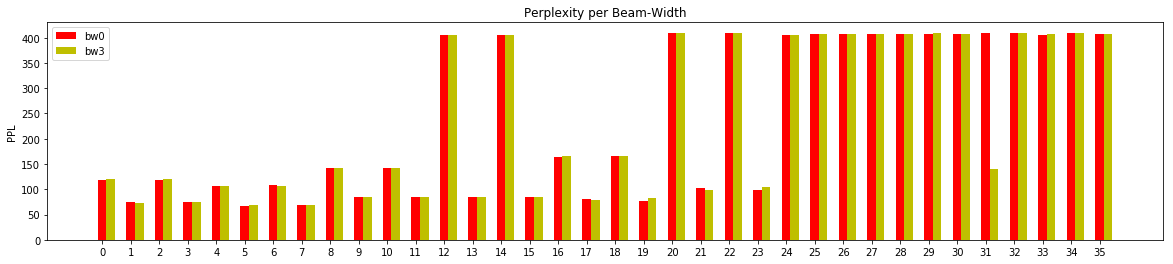
\includegraphics[width=\textheight]{res_run01_bw_ppl}
    \decoRule
    \caption[Results experiment 1 BW-PPL]{Experiment 1 results. Each color represents a beam-width value, x-axis represents the models and y-axis the test perplexity.}
    \label{fig:res_run01_bw_ppl}
\end{figure}
\begin{figure}
    \centering
    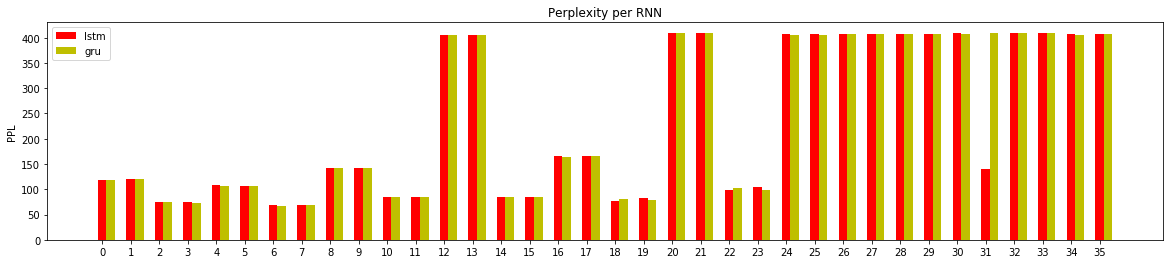
\includegraphics[width=\textheight]{res_run01_c_ppl}
    \decoRule
    \caption[Results experiment 1 C-PPL]{Experiment 1 results. Each color represents a RNN, x-axis represents the models and y-axis the test perplexity.}
    \label{fig:res_run01_c_ppl}
\end{figure}
\begin{figure}
    \centering
    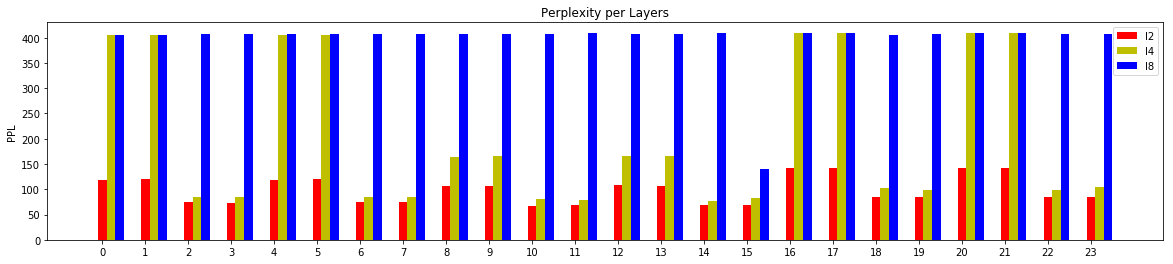
\includegraphics[width=\textheight]{res_run01_l_ppl}
    \decoRule
    \caption[Results experiment 1 L-PPL]{Experiment 1 results. Each color represents a layer value, x-axis represents the models and y-axis the test perplexity.}
    \label{fig:res_run01_l_ppl}
\end{figure}
\begin{figure}
    \centering
    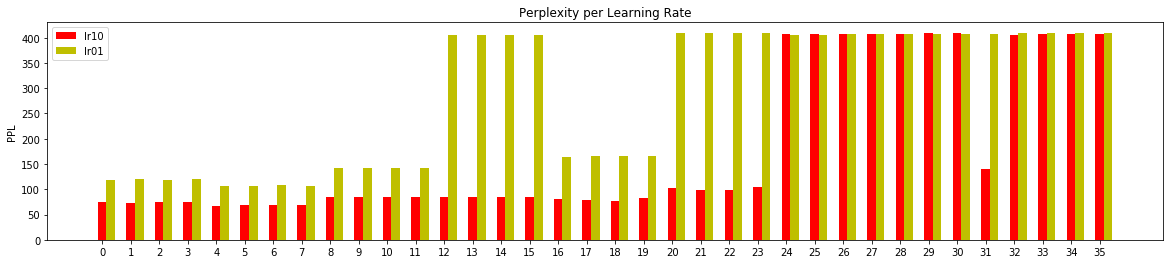
\includegraphics[width=\textheight]{res_run01_lr_ppl}
    \decoRule
    \caption[Results experiment 1 LR-PPL]{Experiment 1 results. Each color represents a learning rate value, x-axis represents the models and y-axis the test perplexity.}
    \label{fig:res_run01_lr_ppl}
\end{figure}
\begin{figure}
    \centering
    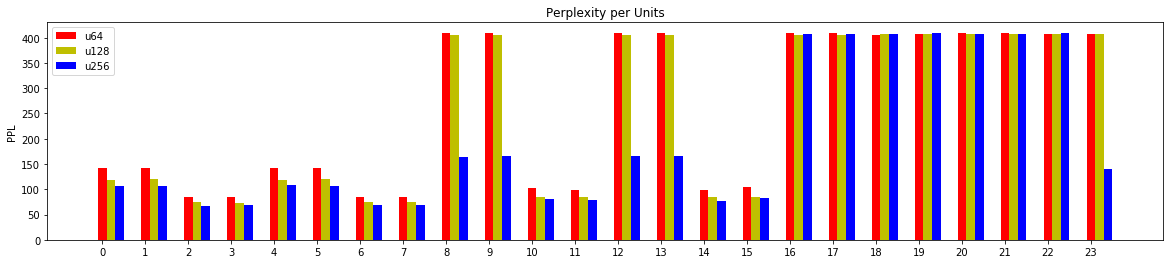
\includegraphics[width=\textheight]{res_run01_u_ppl}
    \decoRule
    \caption[Results experiment 1 U-PPL]{Experiment 1 results. Each color represents an unit value, x-axis represents the models and y-axis the test perplexity.}
    \label{fig:res_run01_u_ppl}
\end{figure}
\end{landscape}

\subsection{Experiment 2 - Limit the vocabulary}
Considering the time needed to train the models in experiment 1, and the fact that the NMT script~\citep{tensorflow.nmt} was thought to use LSTM as RNN model, models using GRU are not tested from experiment 2. This experiment took 31 hours (1 day and 7 hours) and focuses on the importance of the vocabulary in a chatbot model.
Only words appearing more than five times in the training set are kept. As mentioned in Table~\ref{tab:reduce-vocab}, the source vocabulary for a count threshold of 5 contains \num{16456} unique words and the target vocabulary contains \num{16724} unique words.

By comparing Table~\ref{tab:run02-describe} and Table~\ref{tab:run01-describe}, the mean test perplexity in experiment 2 reduced by 52.53\% and the minimum test perplexity reduced by 25.33\%.
\citet{nlp-jurasky-4.4} stated in their defition of perplexity that models can be measured correctly only if their vocabulary is the same. Intuitively, seeing the perplexities reduced is only the result of a smaller vocabulary since the model is less proabable of mistaken. Despite this, the BLEU score kept the same value as during experiment 1.
Limiting the vocabulary might lead to better results, but human evaluation is needed to verify this assumption. Table~\ref{tab:run02-best-models-details} shows the best models for all of the four metrics.

\begin{table}
    \centering
    \caption[Experiment 2 performance statistics]{Experiment 2 performance statistics.}
    \label{tab:run02-describe}
    \begin{tabular}{lrrrrr}
\toprule
{} &   \tabhead{dev\_bleu} &     \tabhead{dev\_ppl} &  \tabhead{test\_bleu} &    \tabhead{test\_ppl} &         \tabhead{Time [s]} \\
\midrule
mean  &   \num{0.030556} &  \num{188.909722} &   \num{0.008333} &  \num{164.751667} &  \num{3107.194444} \\
std   &   \num{0.085589} &  \num{120.715950} &   \num{0.036839} &  \num{111.924972} &  \num{1144.878105} \\
min   &   \num{0.000000} &   \num{64.410000} &   \num{0.000000} &   \num{50.620000} &  \num{1609.000000} \\
25\%   &   \num{0.000000} &   \num{79.350000} &   \num{0.000000} &   \num{63.402500} &  \num{2326.750000} \\
50\%   &   \num{0.000000} &  \num{117.650000} &   \num{0.000000} &   \num{95.975000} &  \num{2602.000000} \\
75\%   &   \num{0.000000} &  \num{334.432500} &   \num{0.000000} &  \num{299.327500} &  \num{4194.750000} \\
max   &   \num{0.400000} &  \num{336.310000} &   \num{0.200000} &  \num{301.840000} &  \num{5204.000000} \\
\bottomrule
\end{tabular}

\end{table}
\begin{table}
    \centering
    \caption[Experiment 2 best models]{Experiment 2 best models with development and testing perplexities and BLEU score metrics.}
    \label{tab:run02-best-models-details}
    \begin{tabular}{rrrr}
        \toprule
        \tabhead{dev\_ppl} & \tabhead{dev\_bleu} & \tabhead{test\_ppl} & \tabhead{test\_bleu}\\
        \midrule
        \multicolumn{4}{l}{\textit{run-20171212014119-norev-l2-u256-clstm-lr10-bw3-voc5}}\\
        \num{64.41} & \num{0.00} & \num{51.19} & \num{0.00}\\
        \hline

        \multicolumn{4}{l}{\textit{run-20171212014119-norev-l2-u256-clstm-lr10-bw0-voc5}}\\
        \num{64.66} & \num{0.10} & \num{50.62} & \num{0.00}\\
        \hline

        \multicolumn{4}{l}{\textit{run-20171212014119-norev-l4-u256-clstm-lr01-bw0-voc5}}\\
        \num{121.43} & \num{0.40} & \num{98.91} & \num{0.00}\\
        \hline

        \multicolumn{4}{l}{\textit{run-20171212014119-norev-l2-u64-clstm-lr01-bw0-voc5}}\\
        \num{115.1} & \num{0.30} & \num{94.60} & \num{0.20}\\

        \bottomrule
    \end{tabular}
\end{table}

Figure~\ref{fig:res_run02_bw_ppl}, Figure~\ref{fig:res_run02_l_ppl}, Figure~\ref{fig:res_run02_lr_ppl} and Figure~\ref{fig:res_run02_u_ppl} show that the model parameters act in the same way on models' performances than during experiment 1. The beam-width and the RNN parameters do not have an impact on the model performance. At contrary, limiting the number of layers, representing tokens with high-dimensionality vectors and preferring a higher learning rate tend to decrease the models' perplexities.

The best model chosen for this experiment is ``run-20171212014119-norev-l2-u256-clstm-lr10-bw0-voc5''. The BLEU scores are still very low, thus the best model decision is mainly based on the test perplexity.

\begin{landscape}
\begin{figure}
    \centering
    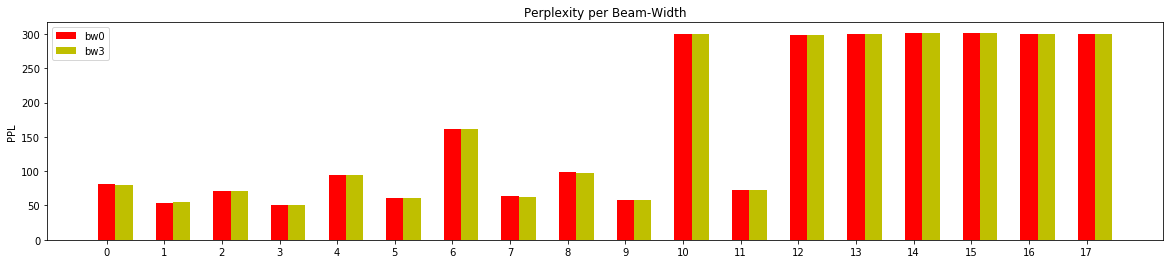
\includegraphics[width=.95\textheight]{res_run02_bw_ppl}
    \decoRule
    \caption[Results experiment 2 BW-PPL]{Experiment 2 results. Each color represents a beam-width value, x-axis represents the experiment number and y-axis the test perplexity.}
    \label{fig:res_run02_bw_ppl}
\end{figure}
% \begin{figure}
%     \centering
%     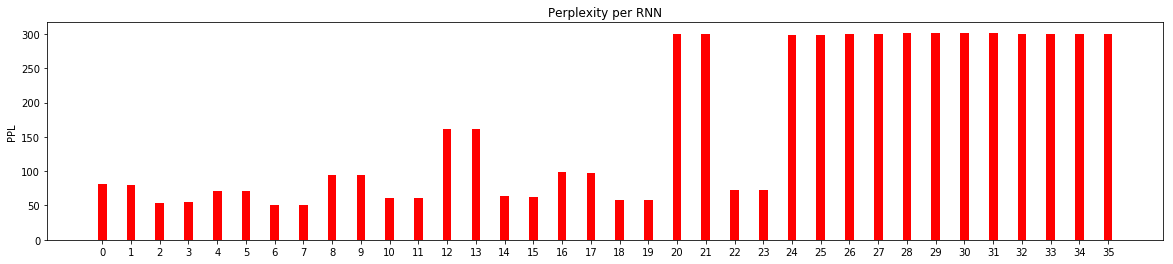
\includegraphics[width=\textheight]{res_run02_c_ppl}
%     \decoRule
%     \caption[Results experiment 2 C-PPL]{Experiment 2 results. Each color represents a RNN, x-axis represents the models and y-axis the test perplexity.}
%     \label{fig:res_run02_c_ppl}
% \end{figure}
\begin{figure}
    \centering
    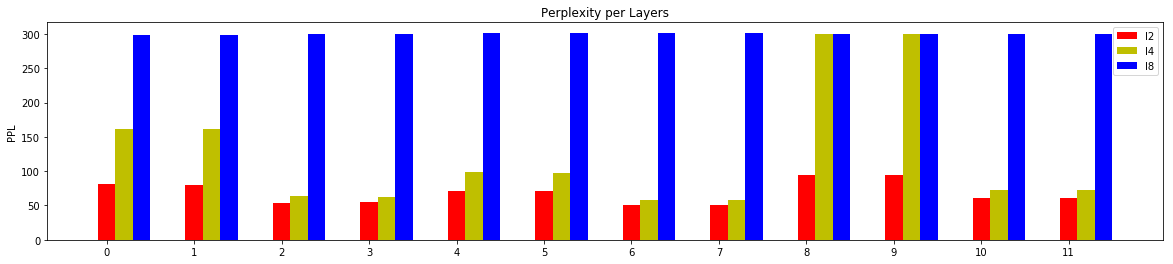
\includegraphics[width=.95\textheight]{res_run02_l_ppl}
    \decoRule
    \caption[Results experiment 2 L-PPL]{Experiment 2 results. Each color represents a layer value, x-axis represents the experiment number and y-axis the test perplexity.}
    \label{fig:res_run02_l_ppl}
\end{figure}
\begin{figure}
    \centering
    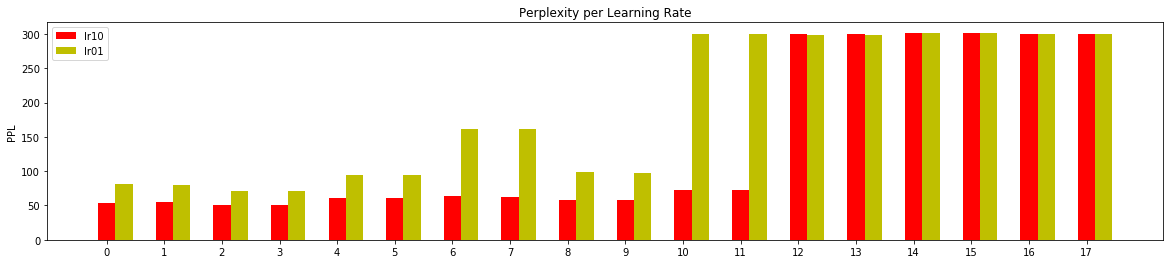
\includegraphics[width=.95\textheight]{res_run02_lr_ppl}
    \decoRule
    \caption[Results experiment 2 LR-PPL]{Experiment 2 results. Each color represents a learning rate value, x-axis represents the experiment number and y-axis the test perplexity.}
    \label{fig:res_run02_lr_ppl}
\end{figure}
\begin{figure}
    \centering
    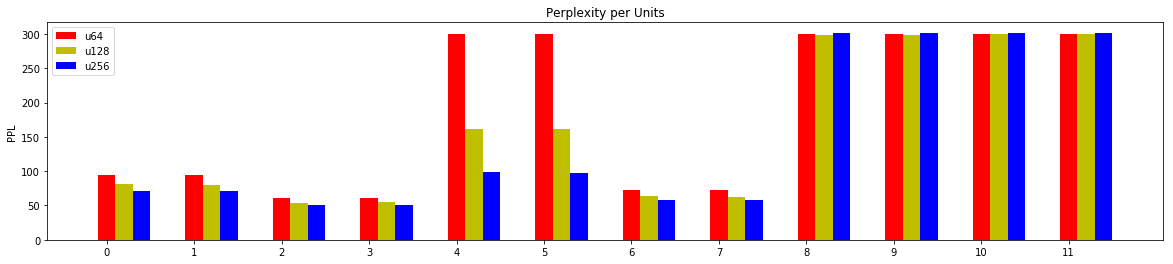
\includegraphics[width=.95\textheight]{res_run02_u_ppl}
    \decoRule
    \caption[Results experiment 2 U-PPL]{Experiment 2 results. Each color represents an unit value, x-axis represents the experiment number and y-axis the test perplexity.}
    \label{fig:res_run02_u_ppl}
\end{figure}
\end{landscape}


\subsection{Experiment 3 - Reversing input sequence}
This experiment focuses on the benefits from inverting the input sequences. This experiment keeps the vocabulary limitation from experiment 2 because multiple papers limited the vocabulary \citep{ecm-1704.01074,1503.02364,1506.05869,1703.01619,tensorflow.nmt} and the time allowed for the experiments is restricted.

By comparing Table~\ref{tab:run02-describe} from experiment 2 and Table~\ref{tab:run03-describe} describing the experiment 3 global performance statistics, there are some improvements. First, although the maximum development BLEU score is smaller by \num{0.1} points, the mean score improved of \num{0.01} points meaning that reversing input sequence might stabilize the models' performances. Secondly, the minimum test perplexity improved by \num{0.27} points and the mean test perplexity improved by \num{4.1} points.

\begin{table}
    \centering
    \caption[Experiment 3 performance statistics]{Experiment 3 performance statistics.}
    \label{tab:run03-describe}
    \begin{tabular}{lrrrrr}
\toprule
{} &   \tabhead{dev\_bleu} &     \tabhead{dev\_ppl} &  \tabhead{test\_bleu} &    \tabhead{test\_ppl} &         \tabhead{Time [s]} \\
\midrule
mean  &   \num{0.036111} &  \num{184.689167} &   \num{0.008333} &  \num{160.852778} &  \num{3476.611111} \\
std   &   \num{0.076168} &  \num{118.469654} &   \num{0.036839} &  \num{109.711937} &   \num{969.338811} \\
min   &   \num{0.000000} &   \num{64.140000} &   \num{0.000000} &   \num{50.350000} &  \num{2121.000000} \\
25\%   &   \num{0.000000} &   \num{78.042500} &   \num{0.000000} &   \num{62.440000} &  \num{2601.500000} \\
50\%   &   \num{0.000000} &  \num{117.200000} &   \num{0.000000} &   \num{96.055000} &  \num{3446.000000} \\
75\%   &   \num{0.025000} &  \num{334.207500} &   \num{0.000000} &  \num{299.252500} &  \num{4125.750000} \\
max   &   \num{0.300000} &  \num{342.640000} &   \num{0.200000} &  \num{305.070000} &  \num{5738.000000} \\
\bottomrule
\end{tabular}

\end{table}

Figure~\ref{fig:res_run03_bw_ppl}, Figure~\ref{fig:res_run03_l_ppl}, Figure~\ref{fig:res_run03_lr_ppl} and Figure~\ref{fig:res_run03_u_ppl} show that the model parameters act in the same way on models' performances than during experiment 1 and experiment 2. When performing the best, the following parameters are used.
\begin{itemize}
    \item Learning rate: 1.0
    \item Number of units: 256
    \item Number of layers: 2
\end{itemize}

Table~\ref{tab:run03-best-models-details} shows the best models for each one of the four metrics. There are only three models because the model ``run-20171212014119-rev-l2-u256-clstm-lr10-bw0-voc5'' has the best development and test perplexity. Thus, it is the best model chosen for this experiment.

\begin{table}
    \centering
    \caption[Experiment 3 best models]{Experiment 3 best models with development and testing perplexity and BLEU score metrics.}
    \label{tab:run03-best-models-details}
    \begin{tabular}{rrrr}
        \toprule
        \tabhead{dev\_ppl} & \tabhead{dev\_bleu} & \tabhead{test\_ppl} & \tabhead{test\_bleu}\\
        \midrule
        \multicolumn{4}{l}{\textit{run-20171212014119-rev-l2-u256-clstm-lr10-bw0-voc5}}\\
        \num{64.41} & \num{0.10} & \num{50.35} & \num{0.00}\\
        \hline

        \multicolumn{4}{l}{\textit{run-20171212014119-rev-l2-u64-clstm-lr10-bw0-voc5}}\\
        \num{76.50} & \num{0.10} & \num{61.02} & \num{0.00}\\
        \hline

        \multicolumn{4}{l}{\textit{run-20171212014119-rev-l2-u64-clstm-lr01-bw0-voc5}}\\
        \num{114.62} & \num{0.30} & \num{94.32} & \num{0.20}\\

        \bottomrule
    \end{tabular}
\end{table}

\begin{landscape}
\begin{figure}
    \centering
    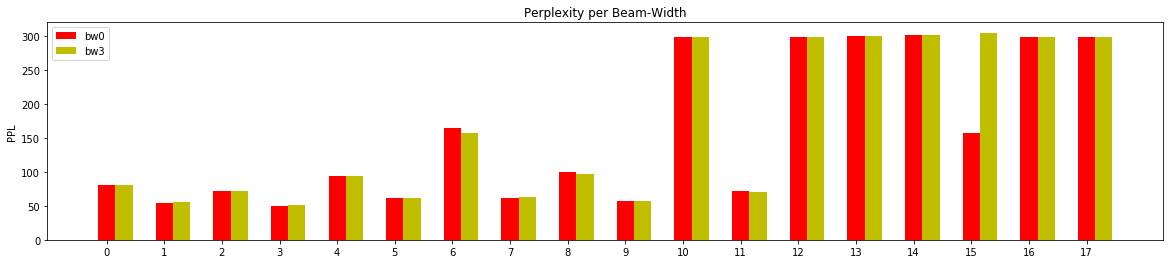
\includegraphics[width=\textheight]{res_run03_bw_ppl}
    \decoRule
    \caption[Results experiment 3 BW-PPL]{Experiment 3 results. Each color represents a beam-width value, x-axis represents the models and y-axis the test perplexity.}
    \label{fig:res_run03_bw_ppl}
\end{figure}
% \begin{figure}
%     \centering
%     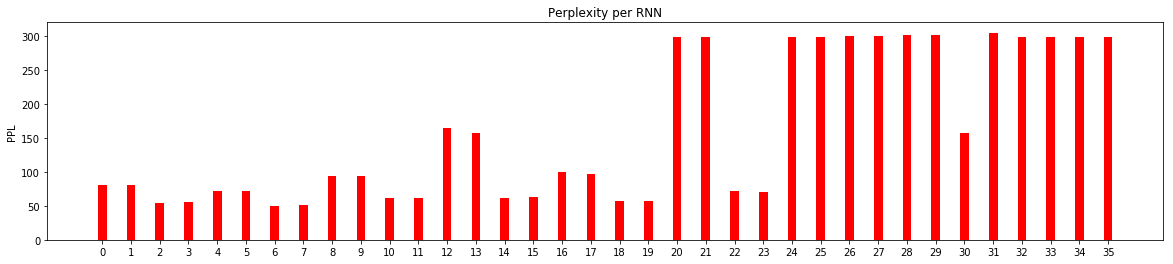
\includegraphics[width=\textheight]{res_run03_c_ppl}
%     \decoRule
%     \caption[Results experiment 3 C-PPL]{Experiment 3 results. Each color represents a RNN, x-axis represents the models and y-axis the test perplexity.}
%     \label{fig:res_run03_c_ppl}
% \end{figure}
\begin{figure}
    \centering
    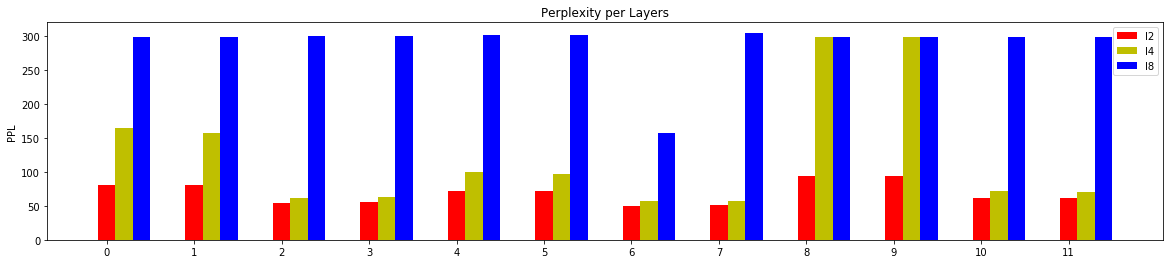
\includegraphics[width=\textheight]{res_run03_l_ppl}
    \decoRule
    \caption[Results experiment 3 L-PPL]{Experiment 3 results. Each color represents a layer value, x-axis represents the models and y-axis the test perplexity.}
    \label{fig:res_run03_l_ppl}
\end{figure}
\begin{figure}
    \centering
    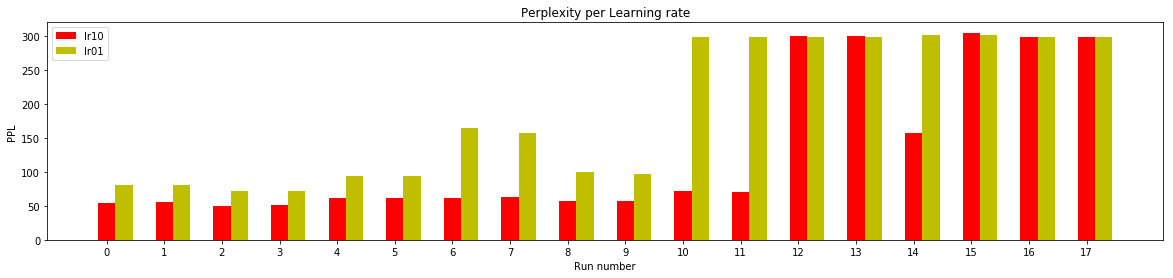
\includegraphics[width=\textheight]{res_run03_lr_ppl}
    \decoRule
    \caption[Results experiment 3 LR-PPL]{Experiment 3 results. Each color represents a learning rate value, x-axis represents the models and y-axis the test perplexity.}
    \label{fig:res_run03_lr_ppl}
\end{figure}
\begin{figure}
    \centering
    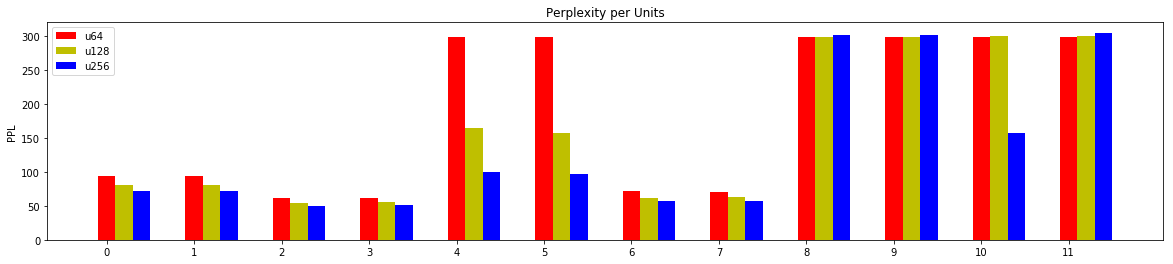
\includegraphics[width=\textheight]{res_run03_u_ppl}
    \decoRule
    \caption[Results experiment 3 U-PPL]{Experiment 3 results. Each color represents an unit value, x-axis represents the models and y-axis the test perplexity.}
    \label{fig:res_run03_u_ppl}
\end{figure}
\end{landscape}

\subsection{Experiment 4 - Attention mechanism}
In their results, \citet{1508.04025} show that for long sentences (between 30 and 70 words), the attention models keep track of the information whereas models without attention show catastrophic results. Moreover, even for short sentences, attention models outperform the model without attention. From that observation, it would be interesting to measure if the attention mechanism increases the performance of the chatbot as well. However, \citet{1506.05869}, constructing a neural conversation machine, reported that adding the attention mechanism \citep{1409.0473} did not improve the perplexity on either training or validation sets.

There are two different attention mechanisms tested in this experiment, namely the ``luong'' (described in Chapter~\ref{Chapter2}, \citet{nmt-phd}) and ``scaled-luong''. The second attention mechanism is almost the same as the first with the exception that it is using a weight normalization inspired from \citet{1602.07868}. Reparameterizing the weights allow the model to converge faster in a stochastic gradient descent.

Experiment 4 only keeps the best value for the parameters \textit{``learning rate''} and \textit{``layers''} found in the three previous experiments. The learning is fixed to \num{1.0} and the number of layers is fixed to \num{2}.
Moreover, since the number of units kept improving the results, instead of testing on ``64'', ``128'' and ``256'', experiment 4 uses the values ``256'', ``384'' and ``512''. In total, during this experiment, 12 models were trained, in 9 hours.

Table~\ref{tab:run04-describe} describes the statistics around the experiment 4 training. Since two parameters were chosen following the three previous experiments, the standard deviation for all of the metrics is significantly reduced. Table~\ref{tab:run04-best-models-details} present the best models of the experiment.
Comparing with the results from the previous experiment, the mean test perplexity increased of \num{2.21} points and the test BLEU metric is now only \num{0.00}. The attention mechanism increases the number of learnable parameters and this might mean that there is not enough data to also train the attention weights.

\begin{table}
    \centering
    \caption[Experiment 4 performance statistics]{Experiment 4 performance statistics.}
    \label{tab:run04-describe}
    \begin{tabular}{lrrrrr}
\toprule
{} &   \tabhead{dev\_bleu} &     \tabhead{dev\_ppl} &  \tabhead{test\_bleu} &    \tabhead{test\_ppl} &         \tabhead{Time [s]} \\
\midrule
mean  &   \num{0.025000} &  \num{67.340000} &        \num{0.0} &  \num{53.509167} &  \num{2796.666667} \\
std   &   \num{0.045227} &   \num{0.840757} &        \num{0.0} &   \num{0.914444} &   \num{267.487411} \\
min   &   \num{0.000000} &  \num{66.070000} &        \num{0.0} &  \num{52.560000} &  \num{2448.000000} \\
25\%   &   \num{0.000000} &  \num{66.835000} &        \num{0.0} &  \num{52.762500} &  \num{2637.750000} \\
50\%   &   \num{0.000000} &  \num{67.220000} &        \num{0.0} &  \num{53.220000} &  \num{2790.000000} \\
75\%   &   \num{0.025000} &  \num{68.050000} &        \num{0.0} &  \num{54.210000} &  \num{2831.750000} \\
max   &   \num{0.100000} &  \num{68.620000} &        \num{0.0} &  \num{55.270000} &  \num{3389.000000} \\
\bottomrule
\end{tabular}

\end{table}

\begin{table}
    \centering
    \caption[Experiment 4 best models]{Experiment 4 best models with development and testing perplexities and BLEU score metrics.}
    \label{tab:run04-best-models-details}
    \begin{tabular}{rrrr}
        \toprule
        \tabhead{dev\_ppl} & \tabhead{dev\_bleu} & \tabhead{test\_ppl} & \tabhead{test\_bleu}\\
        \midrule
        \multicolumn{4}{l}{\textit{run-20171212014119-rev-l2-u384-clstm-lr10-bw3-atscaledluong}}\\
        \num{66.07} & \num{0.00} & \num{52.74} & \num{0.00}\\
        \hline

        \multicolumn{4}{l}{\textit{run-20171212014119-rev-l2-u512-clstm-lr10-bw0-atluong}}\\
        \num{67.00} & \num{0.10} & \num{52.56} & \num{0.00}\\
        \hline

        \multicolumn{4}{l}{\textit{run-20171212014119-rev-l2-u256-clstm-lr10-bw0-atluong}}\\
        \num{68.23} & \num{0.10} & \num{54.20} & \num{0.20}\\

        \bottomrule
    \end{tabular}
\end{table}

Figure~\ref{fig:res_run04_bw_ppl}, Figure~\ref{fig:res_run04_u_ppl} and Figure~\ref{fig:res_run04_at_ppl} illustrates the models behaviour following different parameters' values. As for all other previous experiments, the beam width does not decrease or increase by itself the performance of the models. As suspected, adding more units to the model led to better results. However, the difference in performance from experiments 1, 2 or 3 between 64 units and 256 units is now less visible between 256 units and 512 units. Finally, the different attention strategies do not seem to have an impact themselves on the models' performances.

The model having the best test perplexity is ``run-20171212014119-rev-l2-u512-clstm-lr10-bw0-atluong''.

\begin{landscape}
\begin{figure}
    \centering
    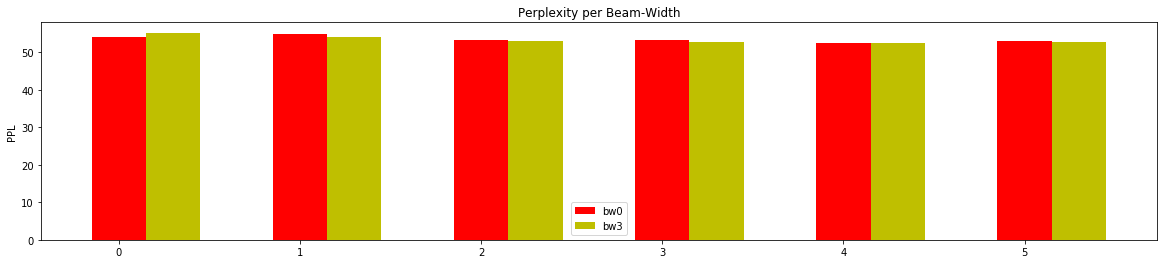
\includegraphics[width=.95\textheight]{res_run04_bw_ppl}
    \decoRule
    \caption[Results experiment 4 BW-PPL]{Experiment 4 results. Each color represents a beam-width value, x-axis represents the models and y-axis the test perplexity.}
    \label{fig:res_run04_bw_ppl}
\end{figure}
\begin{figure}
    \centering
    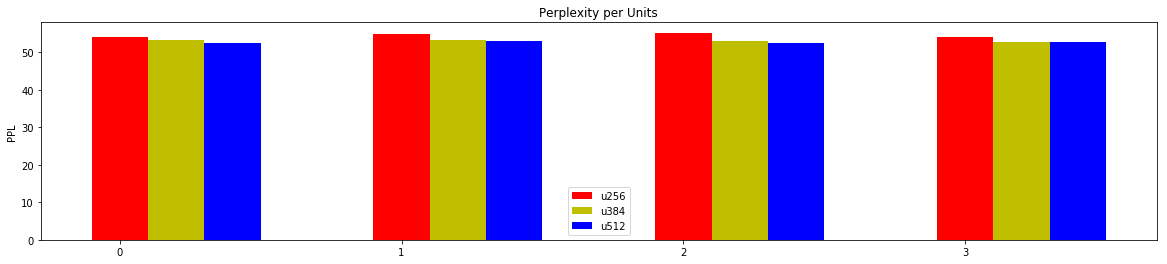
\includegraphics[width=.95\textheight]{res_run04_u_ppl}
    \decoRule
    \caption[Results experiment 4 U-PPL]{Experiment 4 results. Each color represents an unit value, x-axis represents the models and y-axis the test perplexity.}
    \label{fig:res_run04_u_ppl}
\end{figure}
\begin{figure}
    \centering
    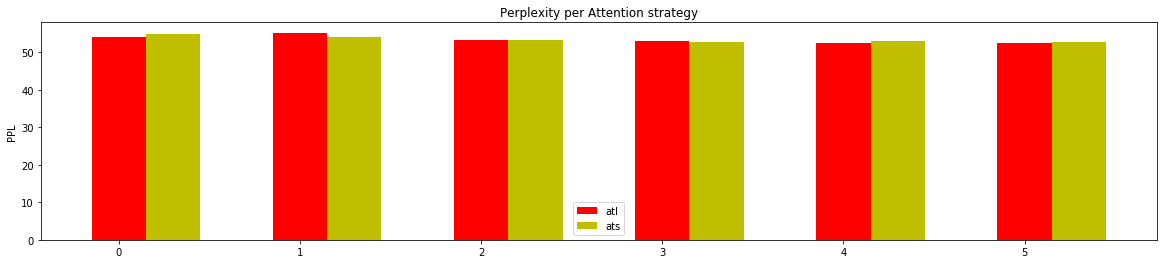
\includegraphics[width=.95\textheight]{res_run04_at_ppl}
    \decoRule
    \caption[Results experiment 4 AT-PPL]{Experiment 4 results. Each color represents a different attention mechanism implementation, x-axis represents the models and y-axis the test perplexity. ``\textit{atl}'' means the attention implementation used is ``luong'' and ``\textit{ats}'' means the attention implementation used is ``scaled\_luong''.}
    \label{fig:res_run04_at_ppl}
\end{figure}
\end{landscape}

\subsection{Experiment 5 - Other dataset splitting ratio}
Since the BLEU score was significantly small for the four previous experiments, this experiment aims at training models using dataset with the 80-10-10 ratio for the training, development and testing sets. The training set contains \num{177023} conversations, the development set contains \num{22095} conversations and the test set contains \num{22161} conversations.

The parameters used for this experiment are the same as in experiment 4, except the number of units fixed to ``512''. In total, this experiment trained 4 different models, in 17 hours.

Table~\ref{tab:run05-describe} shows the different performances obtained during the experiment. By comparing it with Table~\ref{tab:run04-describe}, from experiment 4, the mean test perplexity increased by \num{13.35} points and the min test perplexity increased by \num{12.29} points. However, the BLEU score for both development and test are better than during the previous experiment. Both mean BLEU score is at \num{0.15} point, which is \num{0.12} higher than experiment 4 development BLEU score.

Although the perplexities are worse than in experiment 4, BLEU scores are better and it might mean that besides the lack of evidence that BLEU score is useful to evaluate chatbots, the other dataset might have too small development and test sets.

Besides the evaluation metrics, the time needed to train a model is longer. The mean time is \num{15433.25} whereas, in experiment 4, the mean time was \num{2796.67}, being around 5 times faster than experiment 5.

\begin{table}
    \centering
    \caption[Experiment 5 performance statistics]{Experiment 5 performance statistics.}
    \label{tab:run05-describe}
    \begin{tabular}{lrrrrr}
\toprule
{} &  \tabhead{dev\_bleu} &   \tabhead{dev\_ppl} &  \tabhead{test\_bleu} &   \tabhead{test\_ppl} &          \tabhead{Time [s]} \\
\midrule
mean  &  \num{0.150000} &  \num{65.862500} &   \num{0.150000} &  \num{66.960000} &  \num{15433.250000} \\
std   &  \num{0.057735} &   \num{1.787109} &   \num{0.057735} &   \num{2.302477} &   \num{6984.829579} \\
min   &  \num{0.100000} &  \num{64.260000} &   \num{0.100000} &  \num{64.850000} &   \num{7697.000000} \\
25\%   &  \num{0.100000} &  \num{64.605000} &   \num{0.100000} &  \num{65.457500} &  \num{10628.000000} \\
50\%   &  \num{0.150000} &  \num{65.485000} &   \num{0.150000} &  \num{66.460000} &  \num{15620.500000} \\
75\%   &  \num{0.200000} &  \num{66.742500} &   \num{0.200000} &  \num{67.962500} &  \num{20425.750000} \\
max   &  \num{0.200000} &  \num{68.220000} &   \num{0.200000} &  \num{70.070000} &  \num{22795.000000} \\
\bottomrule
\end{tabular}

\end{table}

\begin{table}
    \centering
    \caption[Experiment 5 best models]{Experiment 5 best models with development and testing perplexities and BLEU score metrics.}
    \label{tab:run05-best-models-details}
    \begin{tabular}{rrrr}
        \toprule
        \tabhead{dev\_ppl} & \tabhead{dev\_bleu} & \tabhead{test\_ppl} & \tabhead{test\_bleu}\\
        \midrule
        \multicolumn{4}{l}{\textit{run-20180119152007-rev-l2-u512-clstm-lr10-bw3-atluong}}\\
        \num{64.26} & \num{0.10} & \num{64.85} & \num{0.10}\\
        \hline

        \multicolumn{4}{l}{\textit{run-20180119152007-rev-l2-u512-clstm-lr10-bw0-atluong}}\\
        \num{66.25} & \num{0.20} & \num{67.26} & \num{0.20}\\
        \hline

        \bottomrule
    \end{tabular}
\end{table}

Table~\ref{tab:run05-best-models-details} presents the best models of this experiments. To keep consistency with the choice of previous best models, ``run-20180119152007-rev-l2-u512-clstm-lr10-bw3-atluong'' is chosen based on the test perplexity even if its BLEU score is interesting.

\subsection{Experiment 6 - GPU performance test}
In the previous chapter, Table~\ref{tab:paperspace-flavors} showed that the ``\textit{V100}'' flavor costs more than 6 times the flavor used for experiments 1 to 5 for a theoretical gain in performance of around 43 times (2.6 teraFLOPS against 112 teraFLOPS). This experiment compares the training time for an exact same model on both flavors to bring the needed information for decision-makers.

Table~\ref{tab:run06-results} illustrates the performance results of the same model trained on different machines. The time gain to use machine that costs 6 times more is around 30\%. Besides the time, the perplexities and the BLEU score are similar.
Even though it is only one measure, this experiment aims at raising awareness on the importance to know very well the model trained to be able to choose correctly the best infrastructure with a limited budget.

\begin{table}
    \centering
    \caption[Experiment 6 GPUs performances results]{Experiment 6 GPUs performances results. V100 is 30\% faster than GPU+ while being 600\% more expensive.}
    \label{tab:run06-results}
    \begin{tabular}{crrrrr}
        \toprule
        \tabhead{Flavor} & \tabhead{dev\_ppl} & \tabhead{dev\_bleu} & \tabhead{test\_ppl} & \tabhead{test\_bleu} & \tabhead{Time [s]}\\
        \midrule
        GPU+ & \num{104.71} & \num{0.5} & \num{83.84} & \num{0.3} & \num{2317}\\
        V100 & \num{105.12} & \num{0.3} & \num{84.23} & \num{0.2} & \num{1596}\\
        \bottomrule
    \end{tabular}
\end{table}

\section{Inference}
\label{sec:inference}
This section illustrates how the chatbots actually converse. Since experiment 6 was just a GPU performance test, only the best models of the five other experiments are used. There are 10 different questions or situations, quite simple, and the chatbots' answers are illustrated in Table~\ref{tab:res-inference}.

First, almost all models answers ``Hello !'' with a ``Hi .'', and all models answer ``No .'' to the question ``Are you a follower or a leader'' and ``What ?'' to the affirmation ``Done .''. This shows that NMT is able to learn some basics independently from the models' parameters.
However, the attention mechanism seems to add more sense to the answers. Typically, in the question ``How are you ?'', both attention-based models answer that they are fine whereas other models do not understand the question.

Secondly, the vocabulary plays an important role in the decoding process and it is witness with all of the ``<unk>'' tokens in questions such as ``What's your name'' or ``Where are you from''. Personal question learned from more than 9k movie characters is indeed difficult and there are high chances that some words in these particular questions appear less than 5 times (which is the threshold to keep or not a word in the vocabulary).

Finally, even if the models presented in this section have respectively the best test perplexity in their experiments, the answers are still not very convincing.

% \begin{table}
% \begin{longtable}{p{.3\textwidth} p{.1\textheight} p{.2\textheight} p{.35\textheight}}
\begin{longtable}{r|cl}

    \caption[Inference results from best experiments' models]{Inference results from best experiments' models. For each experiment, the best model is picked and is given the same 10 questions or situations. E=Experiment. Models used by experiment: (1)~run-20171212014119-norev-l2-u128-clstm-lr10-bw0-voca (2)~run-20171212014119-norev-l2-u256-clstm-lr10-bw0-voc5 (3)~run-20171212014119-rev-l2-u256-clstm-lr10-bw0-voc5 (4)~run-20171212014119-rev-l2-u512-clstm-lr10-bw0-atluong (5)~run-20180119152007-rev-l2-u512-clstm-lr10-bw3-atluong.}
    \label{tab:res-inference}\\
    % \begin{tabular}{l|ll}

    \toprule
    \tabhead{Input} & \tabhead{E} & \tabhead{Output} \\
    \midrule
    \endfirsthead
    \toprule
    \tabhead{Input} & \tabhead{E} & \tabhead{Output} \\
    \midrule
    \endhead
      \midrule
      \multicolumn{3}{r}{\textit{Continued on next page}} \\ % <=======================================
      \bottomrule
    \endfoot % <=======================================
      \bottomrule
    \endlastfoot % <=======================================

    \multirow{5}{*}{Hello !} & 1 & Hi .\\
    & 2 & Hi .\\
    & 3 & Hi .\\
    & 4 & Hi . Hi .\\
    & 5 & I know you are .\\

    \hline
    \multirow{5}{*}{How are you ?} & 1 & What ?\\
    & 2 & I'm not sure .\\
    & 3 & I'm not sure .\\
    & 4 & I'm fine .\\
    & 5 & Fine .\\

    \hline
    \multirow{5}{*}{What's your name ?} & 1 & The man .\\
    & 2 & <unk> .\\
    & 3 & <unk> .\\
    & 4 & Hi .\\
    & 5 & <unk> .\\

    \hline
    \multirow{5}{*}{Where are you from ?} & 1 & The man .\\
    & 2 & <unk> .\\
    & 3 & <unk> .\\
    & 4 & To be .\\
    & 5 & I don't know .\\

    \hline
    \multirow{5}{*}{My name is Rudolf . What is my name ?} & 1 & The man .\\
    & 2 & <unk> .\\
    & 3 & <unk> .\\
    & 4 & Hi . Hi . Hi . Hi . How's business ?\\
    & 5 & <unk> .\\

    \hline
    \multirow{5}{*}{What is your job ?} & 1 &  What ?\\
    & 2 & <unk> .\\
    & 3 & I don't know .\\
    & 4 & My name is John .\\
    & 5 & I don't know .\\

    \hline
    \multirow{5}{*}{Are you a follower or a leader ?} & 1 & No .\\
    & 2 & No .\\
    & 3 & No .\\
    & 4 & No .\\
    & 5 & No .\\

    \hline
    \multirow{5}{*}{What is the color of a yellow car ?} & 1 & You know what ?\\
    & 2 & You know what ?\\
    & 3 & You know what ?\\
    & 4 & It's not a matter of time .\\
    & 5 & I don't know .\\

    \hline
    \multirow{5}{*}{Done .} & 1 &  What ?\\
    & 2 & What ?\\
    & 3 & What ?\\
    & 4 & What ? \\
    & 5 & What ?\\

    \hline
    \multirow{5}{*}{This car was driving too fast !} & 1 &  What ?\\
    & 2 & You were right .\\
    & 3 & What ?\\
    & 4 & What ? \\
    & 5 & I know .\\

    % \end{tabular}
% \end{table}
\end{longtable}


\section{Human evaluation}
In Section~\ref{sec:inference}, having based the best model selection on the test perplexity did not lead to models capable of real conversations. Thus, this section is aiming at showing the best models, not based on the perplexity, but on the perception of comprehension of a human. In other terms, the chatbot is chosen only if its answers make sense.

There are two models having quite good conversation skills amongst all of the trained models, namely ``run-20171212014119-norev-l2-u256-clstm-lr10-bw3-voca'' and ``run-20171212014119-rev-l2-u512-clstm-lr10-bw0-atluong-voc5''. Table~\ref{tab:res-inference-human} shows the conversation skills of both models on the same inference set than in the previous section.

Besides all expectations, the most ``human'' model has neither a limited vocabulary nor reverse input sentence or even attention mechanism. Thus, the perplexity might mean that the optimization is closer to its minima, but it does not mean that the chatbot does its job correctly.

\begin{table}

    \caption[Best models inference from human evaluation]{Inference results from best models from human evaluation. E=Experiment. (1)~run-20171212014119-norev-l2-u256-clstm-lr10-bw3-voca (2)~run-20171212014119-rev-l2-u512-clstm-lr10-bw0-atluong-voc5.}
    \label{tab:res-inference-human}

    \setcellgapes{4pt}
    \makegapedcells

    \begin{tabular}{r|cp{.4\textwidth}}

        \toprule
        \tabhead{Input} & \tabhead{E} & \tabhead{Output} \\
        \midrule

        \multirow{2}{*}{Hello !} & 1 & Hi .\\
        & 2 & Hi . Hi .\\

        \hline
        \multirow{2}{*}{How are you ?} & 1 & Fine .\\
        & 2 & I'm fine .\\

        \hline
        \multirow{2}{*}{What's your name ?} & 1 & Paul .\\
        & 2 & Hi .\\

        \hline
        \multirow{2}{*}{Where are you from ?} & 1 & I don't know .\\
        & 2 & To be .\\

        \hline
        \multirow{2}{*}{My name is Rudolf . What is my name ?} & 1 & Captain .\\
        & 2 & Hi . Hi . Hi . Hi . How's business.\\

        \hline
        \multirow{2}{*}{What is your job ?} & 1 &  What ?\\
        & 2 & My name is John .\\

        \hline
        \multirow{2}{*}{Are you a follower or a leader ?} & 1 & No .\\
        & 2 & No .\\

        \hline
        \multirow{2}{*}{What is the color of a yellow car ?} & 1 & What ?\\
        & 2 & It's not a matter of time .\\

        \hline
        \multirow{2}{*}{Done .} & 1 &  What ?\\
        & 2 & What ?\\

        \hline
        \multirow{2}{*}{This car was driving too fast !} & 1 &  What ?\\
        & 2 & What ? \\

        \bottomrule

    \end{tabular}
\end{table}

Table~\ref{tab:res-inference-training} illustrates inference results from training set samples. The goal of these tests is to observe what the model has learned and if behaviours from unseen data is happening also with seen data.
The models used are the same as in Table~\ref{tab:res-inference-human}. First, the decoded sequences are not the target sequences. Secondly, same patterns are also seen in these conversations. For example, if the model seems to not understand the input, it answers ``\textit{What ?}''.
Lastly, the attention mechanism seems to add more diversity in the model's answers.

\begin{table}

    \caption[Best models from human evaluation inference on training set samples]{Best models from human evaluation inference on training set samples.  E=Experiment. (1)~run-20171212014119-norev-l2-u256-clstm-lr10-bw3-voca (2)~run-20171212014119-rev-l2-u512-clstm-lr10-bw0-atluong-voc5.}
    \label{tab:res-inference-training}

    \setcellgapes{7pt}
    \makegapedcells

    \begin{tabular}{p{.6\textwidth}|cp{.37\textwidth}}

        \toprule
        \tabhead{Input} & \tabhead{E} & \tabhead{Output} \\
        \midrule

        \multirow{2}{.6\textwidth}{Can we make this quick ? Roxanne Korrine and Andrew Barrett are having an incredibly horrendous public break - up on the quad . Again.} & 1 & What ?\\
        & 2 & You were right .\\

        \hline
        \multirow{2}{.6\textwidth}{Well , I thought we'd start with pronunciation , if that's okay with you .} & 1 & No.\\
        & 2 & No .\\

        \hline
        \multirow{2}{.6\textwidth}{Not the hacking and gagging and spitting part . Please .} & 1 & No .\\
        & 2 & You were right .\\

        \hline
        \multirow{2}{.6\textwidth}{You're asking me out . That's so cute . What's your name again ?} & 1 & Hi .\\
        & 2 & Hi .\\

        \hline
        \multirow{2}{.6\textwidth}{No , no , it's my fault -- we didn't have a proper introduction ---} & 1 & No ?\\
        & 2 & No , no , no .\\

        \hline
        \multirow{2}{.6\textwidth}{Cameron .} & 1 &  What ?\\
        & 2 & What ?\\

        \hline
        \multirow{2}{.6\textwidth}{The thing is , Cameron -- I'm at the mercy of a particularly hideous breed of loser . My sister . I can't date until she does .} & 1 & What ?\\
        & 2 & You're not gonna be a killer .\\

        \hline
        \multirow{2}{.6\textwidth}{Why ?} & 1 & Because I don't know what you're talking about .\\
        & 2 & Because I don't know what you're talking about .\\

        \hline
        \multirow{2}{.6\textwidth}{Unsolved mystery . She used to be really popular when she started high school , then it was just like she got sick of it or something .} & 1 &  What ?\\
        & 2 & What happened ?\\

        \hline
        \multirow{2}{.6\textwidth}{Gosh , if only we could find Kat a boyfriend ...} & 1 &  What ?\\
        & 2 & No . \\

        \bottomrule

    \end{tabular}
\end{table}

% interesting inferences:
% \begin{itemize}
%     \item tm_model-20171212014119-l2-u64-clstm-lr10-bw0.infer
%     \item tm_model-20171212014119-l2-u128-cgru-lr10-bw0.infer
%     \item tm_model-20171212014119-l2-u256-cgru-lr10-bw0.infer +1
%     \item tm_model-20171212014119-l2-u256-clstm-lr10-bw0.infer +1
%     \item tm_model-20171212014119-l2-u256-clstm-lr10-bw3.infer +2
%     \item tm_model-20171212014119-l4-u128-cgru-lr10-bw0.infer +0.5 (long sentence)
%     \item tm_model-20171212014119-norev-l2-u256-clstm-lr10-bw0.infer +1 (countries and names are out of the voc)
%     \item tm_model-20171212014119-rev-l2-u512-clstm-lr10-bw0-atluong.infer +2
%     \item tm_model-20171212014119-rev-l2-u512-clstm-lr10-bw0-atscaledluong.infer
%     \item tm_model-20180119152007-rev-l2-u512-clstm-lr10-bw0-atluong.infer +1 (name out of the voc)
% \end{itemize}

% Best parameters :
% LR 1.0
% BW 0 (greedy search best)
% C LSTM
% L 2
% U 512
% voc5
% rev
%
% Run todo:
% - at (luong / scaled_luong), bw (0 / 3), u (256 / 384 / 512) => 12 modeles
